\chapter{ORGANIZAÇÃO DIDÁTICO PEDAGÓGICA}
\label{chap:matriz}

Curso Superior de Engenharia Eletrônica do Câmpus Toledo da UTFPR  é estruturado de acordo com: a Lei nº 9.131, de 24 de novembro de 1995 \cite{Lei:9131:1995}; a Lei nº 9.394, de 20 de dezembro de 1996 \cite{Lei:9394:1996}; a Lei nº 11.184, de 7 de outubro de 2005 \cite{Lei:11.184:2005}; o Estatuto e Regimento Geral da UTFPR \cite{estatutoutfpr}; as Diretrizes Curriculares Nacionais do Curso de Graduação em Engenharia \cite{dcneng}; a Resolução nº 90/2018 – COGEP \cite{cogep90}; e às demais diretrizes e regulamentos internos aplicáveis. A concepção de ensino e aprendizagem do curso, a matriz curricular, os procedimentos de avaliação e os instrumentos de apoio expressos no Projeto Pedagógico de Curso (PPC), são construídos coletivamente e submetidos ao Conselho de Graduação e Educação Profissional (COGEP) para aprovação, em modelo e prazo estabelecido.

Segundo o PPI:

\begin{citacao}
	``A  UTFPR  deve  contribuir  para  o  avanço  conceitual  da educação profissional e tecnológica, tomando como princípio a formação integral do homem,  em  bases  científicas  e  ético-políticas,  entendendo  que  o  exercício  das atividades humanas não se restringe ao caráter produtivo, mas compreende todas as dimensões: social, política, cultural e ambiental'' \cite{ppiutfpr}.
\end{citacao}

Dessa forma, a estrutura curricular do Curso de Engenharia Eletrônica da UTFPR – Campus Toledo possui bases na demanda do mercado regional (veja a \autoref{sec:const}), demanda essa tanto de qualificação profissional, como de características socioeconômicas. Para dar atendimento à demanda do mercado de um profissional com um perfil diferenciado, não só em tecnologia, mas também voltado para o desenvolvimento social e sustentabilidade, a organização do Curso de Engenharia Eletrônica apresenta bases científicas e de gestão de nível superior dimensionada e direcionada às terminalidades da formação do engenheiro.

A organização didático pedagógica deste PPC promove as políticas de ensino e de graduação, previstas nos documentos institucionais norteadores PDI \cite{pdiutfpr} e PPI \cite{ppiutfpr}. As políticas de ensino são as elencadas na seção ``3.3 POLÍTICAS DE ENSINO'' do PDI:

\begin{itemize}
	\item Articulação entre a teoria e a prática;
	\item Desenvolvimento de competências profissionais;
	\item Flexibilidade curricular;
	\item Mobilidade acadêmica;
	\item Articulação entre ensino, pesquisa e extensão.
\end{itemize}

Da mesma forma, as políticas de graduação são elencadas na seção ``3.4 POLÍTICAS DE GRADUAÇÃO'' do PDI:

\begin{itemize}
	\item Flexibilidade curricular;
	\item Articulação com a sociedade;
	\item Mobilidade acadêmica;
	\item Sustentabilidade;
	\item Interculturalidade;
	\item Inovação curricular e metodológica;
	\item Internacionalização.
\end{itemize}

\pdfmarkupcomment{O Curso de Engenharia Eletrônica promove a aprendizagem de conhecimentos estruturados vinculados ao desenvolvimento de competências, em uma dinâmica que enfatiza a prática profissional sem excluir as dimensões sociais e ambientais da qual faz parte. As disciplinas, não mais isoladas, são promotoras do saber, saber fazer e saber ser, se responsabilizando pelo currículo vivo formador de profissionais aptos a mobilizar, integrar e aplicar adequadamente esses conhecimentos. A metodologia do curso envolve processos de participação do estudante que permite a constante construção do conhecimento.}{Retirado do PPC de Tecnologia de alimentos.}

Os conceitos são apresentados a partir dos conhecimentos expostos em livros didáticos, artigos científicos, situações reais e outros materiais bibliográficos pertinentes, conduzidos pela experiência dos docentes. Também são incentivados projetos que permitam a análise reflexiva e o aprendizado da prática profissional pelo discente. Procura-se continuamente estabelecer a interdisciplinaridade relacionando os conteúdos das diversas disciplinas que compõem o curso.

\section{ORGANIZAÇÃO CURRICULAR}

A matriz curricular do curso de Engenharia Eletrônica da UTFPR é estruturada em dez semestres sob o regime de matrícula por disciplina com entrada anual de 88 acadêmicos. Sua carga horária totaliza \pdfmarkupcomment{4060 h}{atualizar ao final} de atividades com conteúdo de natureza profissionalizante, científica, humanística, extensionista e cultural.

A organização da matriz curricular do curso contempla os objetivos de instigar o interesse pela ciência e tecnologia e, ao mesmo tempo, fornece um sólido embasamento para o conteúdo profissionalizante. Isto é alcançado apresentando disciplinas profissionalizantes o mais cedo possível, ao mesmo tempo que o aluno tem uma prévia do que será ministrado adiante no curso através da disciplina de Introdução à Engenharia. A maioria das disciplinas possui carga horária em laboratório, com experimentos realizados nas áreas de física, química e eletrônica desde o primeiro semestre. As disciplinas da área de formação profissionalizante estão presentes em todos os semestres e são desenvolvidas em sua maior parte em laboratório. Especificamente, os conteúdos de computação são apresentados desde o primeiro semestre, enquanto os conteúdos de engenharia elétrica e eletrônica são apresentados desde o terceiro. Além disso, a sequência de pré-requisitos das disciplinas permite a inclusão de atividades interdisciplinares desde o início do curso.

As atividades acadêmicas presenciais são divididas em Atividades Teóricas (AT) e Atividades Práticas (AP). As ATs consistem na apresentação de conteúdos teóricos em sala de aula. Já as APs têm vistas ao desenvolvimento prático dos conteúdos, consistindo de experimentos, atividades de laboratório, ou visitas técnicas. 

Algumas unidades curriculáres também possuem parte da carga horária  em atividades não-presenciais (ANP), que correspondem a processos de ensino e aprendizagem desenvolvidos para além dos tempos e espaços da sala de aula. São mediadas por tecnologias digitais de informação e comunicação, desenvolvidas numa relação dialógica entre docentes e estudantes.

\nomenclature[A]{AT}{Atividades Teóricas}
\nomenclature[A]{AP}{Atividades Práticas}
\nomenclature[A]{ANP}{Atividades não-Presenciais} 

\pdfmarkupcomment{Os projetos pedagógicos dos cursos da UTFPR devem dar ênfase as APs. Para cursos de engenharia, a carga horária de AP, para o conjunto de disciplinas específicas, deve ser de, no mínimo, a metade. Objetiva-se, com isto, formar um profissional diferenciado, apto a lidar com problemas de ordem prática e pronto para lidar com as necessidades imediatas do mercado de trabalho.}{Acho que as diretrizes atuais não delimitam a quantidade de horas práticas}



%A Construção curricular deve responder diretamente aos objetivos formativos. Considerando as metas educacionais para formação profissional percebe-se que para alcança-las os projetos de ensino superior precisam propor mudanças significativas e inovadoras em suas organizações curriculares.

%Assim, é imperativo a construção de currículos inovadores e estrategicamente orientados à aprendizagem significativa, ao desenvolvimento integrado e sustentável, às necessidades, aspirações e expectativas dos alunos e à transformação da realidade em que vivem.

%No início da apresentação da organização curricular deve conter a proposta que fundamenta o curso, pois, são os fundamentos teórico metodológicos que sustentam as decisões sobre a escolha entre uma ou outra matriz curricular. A organização curricular do curso deve apresentar as unidades curriculares agrupadas por áreas de conhecimento, número de períodos, organização de temas transversais, integração horizontal e vertical. Incluir aqui como será desenvolvido no curso o ciclo de humanidades (art. 25 e 26 da Resolução COGEP 90/2018). Descrever se, como e quanto serão utilizados de momentos de aprendizado não presenciais ao longo do curso


\section{MATRIZ CURRICULAR}
\label{sec:matriz}

A matriz curricular do Curso de Engenharia Eletrônica é construída em consonância com os objetivos do curso e da Instituição, atendendo ao perfil do egresso (ver \autoref{sec:perf}), após as discussões dos integrantes do NDE.

Os conteúdos trabalhados devem ter significado aos estudantes, possibilitando uma aprendizagem consistente e significativa. Entende-se que os conhecimentos técnicos não podem estar separados da formação geral e humanística. Os eixos norteadores, destacados, são considerados prioritários e serão desenvolvidos durante toda a trajetória do curso, quais sejam, como Meio ambiente, Ética e Cidadania, Relações Étnico-Raciais, Direitos Humanos, a construção de valores de solidariedade, inclusão, cooperação e respeito à Diversidade.

A partir desta perspectiva, a estruturação curricular do curso seguindo as diretrizes curriculares para os cursos de Engenharia \cite{dcneng}, é embasada em três Núcleos de Conteúdos, com a necessária interligação entre si:

\begin{enumerate}
	\item 	Núcleo de Conteúdos Básicos;
	\item 	Núcleo Conteúdos Profissionalizantes;
	\item 	Núcleo Conteúdos Profissionalizantes Específicos.
\end{enumerate}

Ainda, os discentes do Curso podem desenvolver em \pdfmarkupcomment{conjunto com a Universidade}{atualizar de acordo com a realidade do curso e do campus}:

\begin{itemize}
	\item 	Projetos de Interesse e Inclusão Social;
	\item	Ações para Desenvolvimento Econômico e Responsabilidade Social;
	\item	Atividades de Valorização da diversidade, do meio ambiente, da memória cultural, da produção artística e de patrimônio cultural;
	\item	Projetos de Educação Ambiental e de Desenvolvimento Nacional Sustentável.
\end{itemize}

% Retirado do PPC de campo mourão
A estrutura curricular tem como base a demanda do mercado regional e nacional, sendo norteada pela qualificação profissional e ao atendimento das necessidades socioeconômicas. Para dar atendimento à demanda do mercado por profissionais com um perfil diferenciado, não só em tecnologias emergentes, como também voltado para o desenvolvimento social, a organização do Curso de Bacharelado em Engenharia Eletrônica apresenta bases científicas e de gestão de nível superior dimensionada e direcionada às terminalidades da formação do engenheiro. Estruturada em dez semestres sob o regime de matrícula por disciplina, sua carga horária totaliza \the\value{horasT} h de atividades com conteúdo de natureza profissionalizante, científica, humanística e cultural.

A organização da matriz curricular do curso contempla os objetivos de instigar o interesse pela ciência e tecnologia e, ao mesmo tempo fornecer um sólido embasamento para o conteúdo profissionalizante. Isto é alcançado apresentando disciplinas profissionalizantes o mais cedo possível, ao mesmo tempo em que o aluno tem uma prévia do que será ministrado adiante no curso através da disciplina de Introdução à Engenharia. A maioria das disciplinas possui carga horária em laboratório, com experimentos realizados nas áreas de física, química e eletrônica desde o primeiro semestre. As disciplinas da área de formação profissionalizante estão presentes em quase todos os semestres e são desenvolvidas em sua maior parte em laboratório. Além disso, os conteúdos de engenharia elétrica e eletrônica são apresentados desde o primeiro semestre, buscando a motivação do discente desde o início de sua jornada acadêmica.

As atividades acadêmicas são divididas em atividades teóricas (AT) e práticas (AP), conforme Art. 14 das Diretrizes Curriculares dos Cursos de Graduação Regulares da UTFPR \cite{cogep90}. As ATs correspondem às atividades, de caráter presencial ou não, utilizadas para o desenvolvimento e compreensão de conceitos e de teorias. Já as AP têm vistas às atividades, de caráter presencial ou não, utilizadas para o desenvolvimento prático de conteúdos, tais como: atividades de laboratório, desenvolvimento de projetos, estudos de caso, visitas técnicas, levantamentos em campo, produção de textos, dentre outras.

O Art. 24 em seu parágrafo 1\textordmasculine{} considera que os projetos pedagógicos dos cursos da UTFPR devem dar ênfase a AP. Para cursos de Engenharia, a carga horária de AP deve ser coerente com a formação pretendida. Objetiva-se, com isto, formar um profissional diferenciado, apto a lidar com problemas de ordem prática e pronto para lidar com as necessidades imediatas do mercado de trabalho.

Ainda, o curso desenvolve as ações de: (i) popularização científica e tecnológica; (ii) disseminação tecnológica em escolas do ensino médio e fundamental; (iii) ações para integração com o mundo do trabalho e (iv) projetos de educação ambiental e de desenvolvimento regional sustentável.
%% Fim da cópia

O \autoref{qua:matriz} apresenta a matriz curricular do curso de Engenharia Eletrônica do campus Toledo da UTFPR. \pdfmarkupcomment{As unidades curriculares são codificadas por cores, sendo verde claro: obrigatórias do ciclo de humanidades; verde escuro: optativas do ciclo de humanidades; cinza: optativas específicas; e amarelo: demais unidades curriculares}{Verificar como fica a codificação das cores, até o momento não existe uma orientação.} A seções \ref{sub:reg} à \ref{sub:extch} resumem as informações do referido quadro.

As unidades curriculares do curso, apresentadas na matriz anterior (\autoref{qua:matriz}), apresentam em sua constituição carga horária teórica e prática, com codificação em cada unidade curricular, conforme apresentado na \autoref{fig:legenda}. Portanto, diversas disciplinas promovem a política de ensino ``Articulação entre teoria e prática''.

\begin{figure}[hbt!]
	\centering
	\caption{Codificação das unidades curriculares da Matriz}
	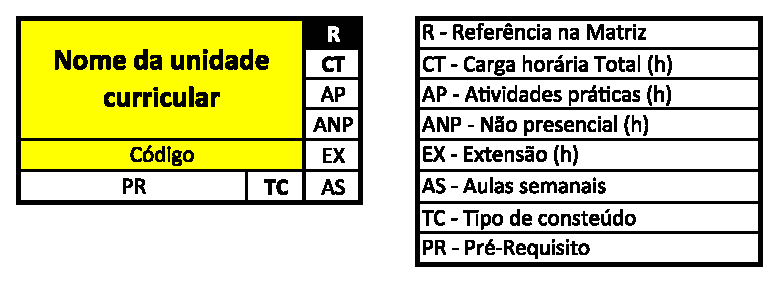
\includegraphics[width=0.6\textwidth]{Caps/Figs/legenda.eps}
	\fonte{\utf}
	\label{fig:legenda}
\end{figure}

\newgeometry{textwidth=200mm,textheight=290mm}
\begin{landscape}
	\begin{quadro}
		\centering
		\caption{Matriz do Curso de Engenharia Eletrônica}
		\includegraphics[width=1.35\textwidth]{Caps/Figs/Matriz_final.eps}
		\fonte{\utf}
		\label{qua:matriz}
	\end{quadro}
\end{landscape}
\restoregeometry



\subsection{Regime Letivo}
\label{sub:reg}

As atividades acadêmicas do curso são de regime semestral, com número mínimo de pré-requisitos, visando melhor consolidação dos conhecimentos nas áreas de atuação do engenheiro eletrônico. A matrícula no curso é realizada por Unidade Curricular. Quanto à matrícula e a periodização serão seguidas as normas institucionais do Regulamento de Organização Didático Pedagógica aplicável ao curso \cite{rodp}.

\subsection{Duração do curso}

O curso de Engenharia Eletrônica possui o período de integralização mínimo em 5 anos (10 períodos, sendo cada período equivalente a um semestre letivo) e máxima em 9 anos (18 semestres), de acordo com o Regulamento da Organização Didático Pedagógica dos Cursos de Graduação da UTFPR \cite{rodp}. A carga horária total é de \the\value{horasT} h. 

Destaca-se que, conforme a Instrução Normativa 02/10 da Instituição \cite{in2:2010:prograd}, uma aula na UTFPR possui 50 minutos. Assim sendo, cada hora das unidade curriculares correspondem a 1,2 aulas. Dessa forma, a cada 15 horas são realizadas 18 aulas.

\subsection{Carga horária de atividades teóricas e práticas}

As atividades teóricas (AT) do curso compreendem \the\value{horasAT} h, correspondendo a \percentagem{\the\value{horasAT}}{\the\value{horasT}} da carga horária total (\the\value{horasT} h). Conforme explicitado na \autoref{sec:matriz}, as ATs correspondem às atividades, de caráter presencial ou não, utilizadas para o desenvolvimento e compreensão de conceitos e de teorias.

\nomenclature[A]{PROGRAD}{Pró-reitoria de Graduação} 

As atividades práticas (AP) do curso compreendem \the\value{horasAP} h, correspondendo a \percentagem{\the\value{horasAP}}{\the\value{horasT}} da carga horária total (\the\value{horasT} h). São atividades de caráter presencial ou não, utilizadas para o desenvolvimento prático de conteúdos, tais como: atividades de laboratório, desenvolvimento de projetos, estudos de caso, visitas técnicas, levantamentos em campo, produção de textos, dentre outras. Além disso, todo ano é promovida a semana acadêmica com enfoque em atividades científicas, minicursos, atividades de extensão, palestras e seminários com profissionais que atuam em áreas pertinentes à formação do discente e outros. Também são promovidas, de acordo com a disponibilidade, visitas técnicas durante o curso.

\subsection{Carga horária de atividades não presenciais}

As atividades não presenciais (ANP) do curso compreendem \the\value{horasANP} h, correspondendo a \percentagem{\the\value{horasANP}}{\the\value{horasT}} da carga horária total (\the\value{horasT} h). As ANPs são distribuídas em diversas disciplinas estratégicas visando fomentar a cultura de ensino à distância no corpo discente e docente, gerando assim maturidade para esse processo de ensino-aprendizagem. Essa carga horária deve ser planejada pelos docentes, observando, necessariamente, a mediação por Tecnologias da Informação e Comunicação (TICS), assim como atender a regulamentação definida na Resolução nº 39/2019 – COGEP \cite{cogep39}. 

Segundo portaria de MEC N\textordmasculine{} 2.117, de 6 de dezembro de 2019 \cite{portaria2117mec}, as instituições de ensino poderão ofertar disciplinas em no \pdfmarkupcomment{máximo 40\%}{inserir um quadro demonstrativo? A utfpr prevê ainda 20\%?} de sua carga horária total do curso. A principal ferramenta de Tecnologia de informação e comunicação (TIC) para a oferta desta modalidade é o sistema MOODLE. Para que uma disciplina ocorra desta maneira deve estar previsto em plano de ensino e ser aprovado por colegiado competente. Entretanto, em caso de ausência do docente por motivo previsto ou não previsto (como acidentes, doenças, falecimentos, dentre outros) a aula pode ser antecipada ou reposta por meio de uma atividade não presencial a distância desde que seja aprovada pelo coordenador do curso conforme Resolução n\textordmasculine 084/17 do COGEP \cite{cogep84}.

\nomenclature[A]{AD}{Aulas à distência}
\nomenclature[A]{ANPD}{Atividades não presenciais}

\subsection{Carga horária do Estágio Curricular Obrigatório}

Segundo as Diretrizes Curriculares Nacionais dos Cursos de Graduação em Engenharia \cite{dcneng}, em seu artigo 11, ``a formação  do  engenheiro  inclui,  como  etapa  integrante da  graduação, as práticas reais, entre as quais o estágio curricular obrigatório sob supervisão direta do curso''. Aliado a essa diretriz, a UTFPR estabelece, na Resolução Conjunta COGEP-COEMP N\textordmasculine{} 01/2020, de 02 de junho de 2020 \cite{cogepcoemp1:2020}, que a carga horária mínima de estágio obrigatório para os cursos da UTFPR deve ser de no mínimo 400 horas, sendo esse o mesmo valor adotado pelo curso de Engenharia Eletrônica.

\nomenclature[A]{COEMP}{Conselho de Ralações Empresariais e comunitárias}

%\subsection{Carga horária do TCC}

%O TCC tem uma carga total de 144 horas-aula, a carga horária é dividida igualmente nas disciplinas de TCC 1 e TCC 2.

%\subsection{Carga horária de Atividade complementares}

%\pdfmarkupcomment{Verificar se as Atividade complementares continuarão.}{segundo as DCNs, deve-se manter}

\subsection{Carga horária das Atividades de Extensão}
\label{sub:extch}

A curricularização da Extensão no curso, é desenvolvida como uma possibilidade de aplicação de um conjunto de conhecimentos desenvolvidos durante as atividades de ensino e pesquisa e ofertada para a comunidade universitária da UTFPR, à comunidade no entorno direto da Universidade e às regiões circunvizinhas.

As atividades de Extensão enfocam a observação da realidade, tratada com o objetivo de produzir impacto junto à comunidade visando o desenvolvimento regional sustentável. Estarão organizadas em torno de programas ou projetos, sendo incluídas no projeto individual de algumas disciplinas, totalizando \the\value{horasEXT} h, representando \percentagem{\the\value{horasEXT}}{\the\value{horasT}} da carga horária total do curso.

\subsection{Carga horária dos Núcleos de Conteúdos}

Conforme estabelece as Diretrizes Curriculares Nacionais para os cursos Engenharia, existem três núcleos de conteúdo: (i) Básicos; (ii) Profissionalizantes e (iii) Profissionalizantes Específicos. A carga horária desses núcleos no âmbito do curso de Engenharia Eletrônica é mostrada no \autoref{tab:nucleos}.

\begin{table}
	\centering
	\caption[Carga horária dos núcleos de conteúdo]{Carga horária dos núcleos de conteúdo}        
    \label{tab:nucleos}
	\begin{tabularx}{0.7\textwidth}{>{\centering\arraybackslash}X >{\centering\arraybackslash}X >{\centering\arraybackslash}X }\toprule
	\textbf{Núcleo}					& \textbf{Carga horária (h)}	& \textbf{\% da carga horária total}	\\ \midrule 
	Básico							& \the\value{horasB}			& \percentagem{\the\value{horasB}}{\the\value{horasT}}	\\ \rowcolor{gray!10}
	Profissionalizante				& \the\value{horasPR}			& \percentagem{\the\value{horasPR}}{\the\value{horasT}}	\\ 
	Profissionalizante Específico	& \the\value{horasPE}			& \percentagem{\the\value{horasPE}}{\the\value{horasT}}	\\ \bottomrule
	\end{tabularx}
\end{table}

\subsection{Carga horária do ciclo de humanidades}

A fim de contribuir para uma formação mais humanística de seus egressos, os Projetos Pedagógicos dos Cursos de graduação da UTFPR devem estabelecer em sua estrutura curricular um ciclo de humanidades \cite{cogep90}. No curso de Engenharia Eletrônica o ciclo de humanidades é estabelecido em \the\value{horasH} h, correspondendo a \percentagem{\the\value{horasH}}{\the\value{horasT}} da carga horária total do curso.

\section{CONTEÚDOS CURRICULARES}

Esta seção descreve os componentes curriculares por período, as unidades curriculares obrigatórias, optativas e eletivas, demonstrando a totalização das cargas horárias.  A composição da distribuição gradual dos períodos e áreas de conhecimento é apresentado em uma sequência didática lógica demonstrando a integração entre os componentes curriculares. Também é descrito como está estruturado o ciclo de humanidades (grupo de unidades curriculares da área de humanidades exigido pela Resolução 90 do COGEP \cite{cogep90}).

\subsection{Unidades Curriculares do Primeiro Período}

Este período do curso, historicamente, apresenta-se como um dos semestres mais difíceis e desafiadores para o corpo discente. Isto pode estar relacionado ao próprio momento em que o discente se encontra, buscando se adaptar a uma nova realidade, muitas das vezes experimentando o conflito entre a gestão da liberdade pessoal e a necessidade de se disciplinar frente às atividades acadêmicas. Em outra perspectiva, a turma do Primeiro Período geralmente apresenta grande diversidade de cultura e formação básica, o que torna importante a implementação de momentos de nivelamento e ambientação que propiciem um melhor fluxo de desenvolvimento das disciplinas e, consequentemente, seu melhor aproveitamento.

Desta forma, o Primeiro Período possui disciplinas que buscam e ambientar o discente ao curso, tais como ``Introdução à Engenharia'' e ``Computação 1''.

Adicionalmente, este período é o início do alicerce para as fundamentações matemáticas necessárias para o bom engenheiro eletrônico. Essa fundamentação se estende até o quarto período onde, a partir de então, as unidades curriculares específicas e profissionalizantes se iniciam.

%As unidades curriculares do Primeiro Período são \listaUC{1}{Dados/unidadesCurriculares.csv}, totalizando \the\value{horasP1} h. A \autoref{tab:per1} representa a distribuição das unidades curriculares do primeiro período do curso de Engenharia Eletrônica. Dessa forma,\listaUC{1}{Dados/unidadesCurriculares.csv}, totalizam \the\value{horasP1} h.

Os conteúdos curriculares do primeiro período estão listados na \autoref{tab:per1}. Adicionalmente, a estrutura de cada unidade curricular é apresentada em quadros: \listaUC{1}{Dados/unidadesCurriculares.csv}.

% tabela de unidades curriculares do primeiro período
\begin{table}[!htb]
	\centering\footnotesize
	\caption{Conteúdos curriculares do Primeiro Período}
	\label{tab:per1}
	\tabelaPeriodo{1}{Dados/unidadesCurriculares.csv}
	\fonte{Autoria própria}
\end{table}

\imprimeEmentas{1}{Dados/unidadesCurriculares.csv}\clearpage



\subsection{Unidades Curriculares do Segundo Período}

Os conteúdos curriculares do segundo período estão listados na \autoref{tab:per2}. Adicionalmente, a estrutura de cada unidade curricular é apresentada em quadros: \listaUC{2}{Dados/unidadesCurriculares.csv}.

% tabela de unidades curriculares do segundo período
\begin{table}[!htb]
	\centering\footnotesize
	\caption{Conteúdos curriculares do Segundo Período}
	\label{tab:per2}
	\tabelaPeriodo{2}{Dados/unidadesCurriculares.csv}
	\fonte{Autoria própria}
\end{table}

\imprimeEmentas{2}{Dados/unidadesCurriculares.csv}\clearpage

\subsection{Unidades Curriculares do Terceiro Período}

Os conteúdos curriculares do terceiro período estão listados na \autoref{tab:per3}. Adicionalmente, a estrutura de cada unidade curricular é apresentada em quadros: \listaUC{3}{Dados/unidadesCurriculares.csv}.

% tabela de unidades curriculares do terceiro período
\begin{table}[!htb]
	\centering\footnotesize
	\caption{Conteúdos curriculares do Terceiro Período}
	\label{tab:per3}
	\tabelaPeriodo{3}{Dados/unidadesCurriculares.csv}
	\fonte{Autoria própria}
\end{table}

\imprimeEmentas{3}{Dados/unidadesCurriculares.csv}\clearpage

\subsection{Unidades Curriculares do Quarto Período}

Os conteúdos curriculares do quarto período estão listados na \autoref{tab:per4}. Adicionalmente, a estrutura de cada unidade curricular é apresentada em quadros: \listaUC{4}{Dados/unidadesCurriculares.csv}.

% tabela de unidades curriculares do quarto período
\begin{table}[!htb]
	\centering\footnotesize
	\caption{Conteúdos curriculares do Quarto Período}
	\label{tab:per4}
	\tabelaPeriodo{4}{Dados/unidadesCurriculares.csv}
	\fonte{Autoria própria}
\end{table}

\imprimeEmentas{4}{Dados/unidadesCurriculares.csv}\clearpage

\subsection{Unidades Curriculares do Quinto Período}

Os conteúdos curriculares do quinto período estão listados na \autoref{tab:per5}. Adicionalmente, a estrutura de cada unidade curricular é apresentada em quadros: \listaUC{5}{Dados/unidadesCurriculares.csv}.

% tabela de unidades curriculares do quinto período
\begin{table}[!htb]
	\centering\footnotesize
	\caption{Conteúdos curriculares do Quinto Período}
	\label{tab:per5}
	\tabelaPeriodo{5}{Dados/unidadesCurriculares.csv}
	\fonte{Autoria própria}
\end{table}

\imprimeEmentas{5}{Dados/unidadesCurriculares.csv}\clearpage

\subsection{Unidades Curriculares do Sexto Período}

Os conteúdos curriculares do sexto período estão listados na \autoref{tab:per6}. Adicionalmente, a estrutura de cada unidade curricular é apresentada em quadros: \listaUC{6}{Dados/unidadesCurriculares.csv}.

% tabela de unidades curriculares do sexto período
\begin{table}[!htb]
	\centering\footnotesize
	\caption{Conteúdos curriculares do Sexto Período}
	\label{tab:per6}
	\tabelaPeriodo{6}{Dados/unidadesCurriculares.csv}
	\fonte{Autoria própria}
\end{table}

\imprimeEmentas{6}{Dados/unidadesCurriculares.csv}\clearpage

\subsection{Unidades Curriculares do Sétimo Período}

Os conteúdos curriculares do sétimo período estão listados na \autoref{tab:per7}. Adicionalmente, a estrutura de cada unidade curricular é apresentada em quadros: \listaUC{7}{Dados/unidadesCurriculares.csv}.

% tabela de unidades curriculares do sexto período
\begin{table}[!htb]
	\centering\footnotesize
	\caption{Conteúdos curriculares do Sétimo Período}
	\label{tab:per7}
	\tabelaPeriodo{7}{Dados/unidadesCurriculares.csv}
	\fonte{Autoria própria}
\end{table}

\imprimeEmentas{7}{Dados/unidadesCurriculares.csv}\clearpage

\subsection{Unidades Curriculares do Oitavo Período}

Os conteúdos curriculares do oitavo período estão listados na \autoref{tab:per8}. Adicionalmente, a estrutura de cada unidade curricular é apresentada em quadros: \listaUC{8}{Dados/unidadesCurriculares.csv}.

% tabela de unidades curriculares do sexto período
\begin{table}[!htb]
	\centering\footnotesize
	\caption{Conteúdos curriculares do Oitavo Período}
	\label{tab:per8}
	\tabelaPeriodo{8}{Dados/unidadesCurriculares.csv}
	\fonte{Autoria própria}
\end{table}

\imprimeEmentas{8}{Dados/unidadesCurriculares.csv}\clearpage

\subsection{Unidades Curriculares do Nono Período}

Os conteúdos curriculares do nono período estão listados na \autoref{tab:per9}. Adicionalmente, a estrutura de cada unidade curricular é apresentada em quadros: \listaUC{9}{Dados/unidadesCurriculares.csv}.

% tabela de unidades curriculares do sexto período
\begin{table}[!htb]
	\centering\footnotesize
	\caption{Conteúdos curriculares do Nono Período}
	\label{tab:per9}
	\tabelaPeriodo{9}{Dados/unidadesCurriculares.csv}
	\fonte{Autoria própria}
\end{table}

\imprimeEmentas{9}{Dados/unidadesCurriculares.csv}\clearpage

\subsection{Unidades Curriculares do Décimo Período}

Os conteúdos curriculares do décimo período estão listados na \autoref{tab:per10}. Adicionalmente, a estrutura de cada unidade curricular é apresentada em quadros: \listaUC{10}{Dados/unidadesCurriculares.csv}.

% tabela de unidades curriculares do sexto período
\begin{table}[!htb]
	\centering\footnotesize
	\caption{Conteúdos curriculares do Décimo Período}
	\label{tab:per10}
	\tabelaPeriodo{10}{Dados/unidadesCurriculares.csv}
	\fonte{Autoria própria}
\end{table}

\imprimeEmentas{10}{Dados/unidadesCurriculares.csv}\clearpage